\documentclass[utf8]{beamer}
\usepackage{ctex}
\usetheme{Brief}
\usepackage{graphicx}
\usepackage{hyperref}%
\usepackage{marvosym}
\titlegraphic{
\includegraphics[height=10ex]{fig/ZJUBLUE.eps}}
\logo{
\includegraphics[width=2cm]{fig/logo2.eps}}
\title{带校徽的展示模板}
\subtitle{简洁主题}
\author{王二}
\institute{\href{mailto:Feb14@163.com}{\Letter Feb14\MVAt163.com}\\\vspace{1ex}人文与社会科学学院}
\subject{专业}

\begin{document}
\begin{frame}
	\titlepage
	\thispagestyle{empty}
\end{frame}
\section{大纲}
\begin{frame}
	\frametitle{\mylogo 大纲}
\tableofcontents

\end{frame}
\section{块环境}
\begin{frame}
\frametitle{\mylogo 块环境}
	\begin{block}{\vskip1ex 块环境}
		这是块环境的内容,比如插入欧拉公式:
		\begin{equation}
			e+v=2\cdot r
		\end{equation}
	\end{block}
\end{frame}
\section{列表}
\begin{frame}
	\frametitle{\mylogo 列表}
	\begin{block}{无序列表}
	\begin{itemize}
		\item 这是一个无序列表
		\item 这是无序列表的第二项
	\end{itemize}
	\end{block}
	\begin{block}{有序列表}
		\begin{enumerate}	
		\item 这是一个有序列表
		\item 这是一个有序列表的第二项
	\end{enumerate}
	\end{block}
\end{frame}
\section{图文排版}
\begin{frame}{\mylogo 项目负责人}
	\begin{columns}
		\begin{column}{.4\linewidth}
			\begin{figure}[h]
				\centering
				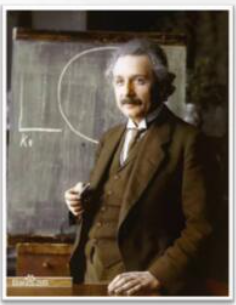
\includegraphics[width=0.5\linewidth]{fig/p1}
				\caption{爱因斯坦}
				\label{fig:1}
			\end{figure}	
		\end{column}
		\begin{column}{.7\linewidth}	
		{\usebeamercolor{block title}\usebeamerfont{block title}阿尔伯特$\cdot$爱因斯坦}
		\begin{itemize}
		\item 出生于德国巴登-符腾堡州乌尔姆市
		\item \alert{毕业于苏黎世联邦理工学院}
		\item 现代物理学家
		\item 代表作《非欧几里德几何和物理学》《统一场论》《我的世界观》等
		\end{itemize}
	\end{column}
\end{columns}
\vspace{3ex}
{\usebeamerfont{block title}主要成就}
\begin{itemize}
\item 提出\alert{光量子假说},解决了\alert{光电效应问题}
\item 创立了狭义相对论、广义相对论等
\item 被美国《时代周刊》评选为\alert{“世纪伟人”}
\end{itemize}
\footnote{图源\href{https://www.cc98.org/topic/4979847}{https://www.cc98.org/topic/4979847}}
\end{frame}

\end{document}
